% 90-10(90쪽) — 원에 내접하는 사각형 ABCD(원문 「오른쪽 그림」). 스캔 화질이 낮아 TikZ 로 다시 그림.
% 라벨은 원문 것만 — 네 점 이름, $\seg{AC}=6\sqrt{2}$, $25^\circ$, $20^\circ$, $70^\circ$.
% $\seg{BD}$(답)의 길이는 적지 않는다. $\seg{AC}$ 는 원문처럼 점선.
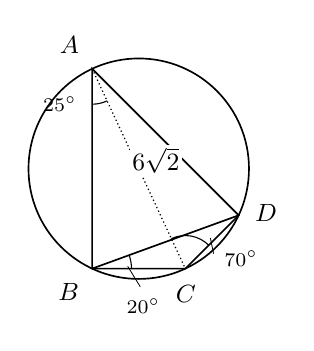
\begin{tikzpicture}[line width=0.6pt]
  \coordinate (A) at (-0.592,1.269);
  \coordinate (B) at (-0.592,-1.269);
  \coordinate (C) at (0.592,-1.269);
  \coordinate (D) at (1.269,-0.592);
  \draw (0,0) circle (1.400);
  \draw (A) -- (B) -- (C) -- (D) -- cycle;
  \draw (B) -- (D);
  \draw[densely dotted, line width=0.45pt] (A) -- (C);
  % $25^\circ$ = $\angle\pt{BAC}$
  \draw[line width=0.4pt] (-0.592,0.819) arc (270:295:0.45);
  \node[font=\scriptsize, anchor=east] at (-0.66,0.82) {$25^\circ$};
  % $20^\circ$ = $\angle\pt{DBC}$
  \draw[line width=0.4pt] (-0.092,-1.269) arc (0:20:0.50);
  \draw[line width=0.3pt] (0.02,-1.50) -- (-0.14,-1.24);
  \node[font=\scriptsize, anchor=north] at (0.06,-1.52) {$20^\circ$};
  % $70^\circ$ = $\angle\pt{ACD}$
  \draw[line width=0.4pt] (0.889,-0.972) arc (45:115:0.42);
  \draw[line width=0.3pt] (0.95,-1.08) -- (0.91,-0.88);
  \node[font=\scriptsize, anchor=west] at (0.96,-1.14) {$70^\circ$};
  \node[font=\small, fill=white, inner sep=1pt] at (0.218,0.102) {$6\sqrt{2}$};
  \node[font=\small, anchor=south east] at (-0.63,1.33) {$\pt{A}$};
  \node[font=\small, anchor=north east] at (-0.63,-1.33) {$\pt{B}$};
  \node[font=\small, anchor=north] at (0.60,-1.36) {$\pt{C}$};
  \node[font=\small, anchor=west] at (1.35,-0.56) {$\pt{D}$};
\end{tikzpicture}
